\documentclass[oneside,12pt]{book}
% oneside - onesided print

%\usepackage[czech]{babel}
\usepackage[utf8]{inputenc}
\usepackage[a4paper,width=150mm,top=25mm,bottom=30mm]{geometry}
\usepackage[backend=biber,style=numeric,sorting=none]{biblatex}
\usepackage{setspace, enumitem, amsmath, amsfonts, amsthm, amssymb, graphicx, soul, float, multirow, hyperref}
\usepackage{xcolor, listings, csquotes, wrapfig}

% Page number at the end of page and no chapter name in the header
\pagestyle{plain}

\setstretch{1.5}

\setcounter{secnumdepth}{3}

\bibliography{references}

\definecolor{keywords}{rgb}{0,0,0.7}

\lstset{
columns=fullflexible,
keywordstyle=\color{keywords},
frame=lines,
language=Python,
%numbers=left,
%numbersep=5pt,
basicstyle=\small,
%numberstyle=\footnotesize\color{Gray},
commentstyle=\it\footnotesize\color{Gray}
}

\newenvironment{boldenv}{\bfseries}{}

\newcommand\norm[1]{\left\lVert#1\right\rVert}

\theoremstyle{definition}
\newtheorem{defn}{Definition}[section]

\DeclareMathOperator*{\argmax}{arg\,max}
\DeclareMathOperator*{\argmin}{arg\,min}

\begin{document}
    \pagenumbering{gobble}

    \begin{titlepage}
    \begin{boldenv}
        \begin{center}
            \vspace*{20pt}
            \LARGE
            University of West Bohemia \\
            \vspace*{5pt} Faculty of Applied Sciences  \\
            \vspace*{5pt} Department of Cybernetics\\

            \vfill
            \huge
            MASTER THESIS

            \vfill

        \end{center}
        \begin{flushleft}
            \Large
            PILSEN, 2020
            \hfill
            JAN BENEŠ
        \end{flushleft}
    \end{boldenv}
\end{titlepage}

    Před svázáním místo této stránky \fbox{vložit zadání práce} s podpisem děkana.
    \newpage

    \vspace*{20pt}
\begin{center}
    \underline{Declaration of Authorship}
\end{center}

I, Jan Beneš, declare that this thesis titled, “Automatic face recognition using neural networks” and the work 
presented in it are my own.

I confirm that:
\begin{itemize}
    \item Where I have consulted the published work of others, this is always clearly attributed.
    \item Where I have quoted from the work of others, the source is always given.
    With the exception of such quotations, this thesis is entirely my own work.
    \item I have acknowledged all main sources of help.
\end{itemize}

    \newpage

    \vspace*{20pt}
\noindent
{\LARGE
\textbf{Acknowledgements}
}
\vspace*{0.5em}
\newline
TODO

    \section*{Abstract}
The goal of this study is to design and implement an end-to-end facial recognition system.
The first part is focused on a general overview of modern methods followed by an in-depth description of
state-of-the-art research of loss functions.
The emphasis is being put on the ArcFace loss as it is the research which forms the basis of the facial recognition
system implemented in this thesis.
The second part deals with the design and implementation of the system.
The end of the text contains a comparison with a commercial algorithm.
The performance was evaluated on a dataset which was created from the recordings of evening news on the czech public
television broadcast (Česká Televize).

\vspace{1cm}

\subsection*{Key words}
Machine learning, facial recognition, identification, verification, convolutional neural networks, loss functions,
ArcFace

\vfill

\section*{Abstrakt}
Cílem této práce je návrh a implementace systému rozpoznávání obličeje.
V první části je poskytnut přehled moderních metod, na který navazuje podrobný rozbor výzkumu ztrátových funkcí.
Důraz je kladen na ztrátovou funkci ArcFace.
Tato funkce byla použita při trénování modelu, jenž tvoří jádro systému implementovaného v rámci této práce.
Druhá část práce obsahuje návrh a popis implementace systému.
V závěru je systém porovnán s komerčním algoritmem.
Vyhodnocení proběhlo na datasetu, jenž byl vytvořen ze záznamu večerních zpráv České Televize.

\vspace{1cm}

\subsection*{Klíčová slova}
Strojové učení, rozpoznávání obličeje, identifikace, verifikace, konvoluční neuronové sítě, ztrátové funkce, ArcFace

    \tableofcontents

    \pagenumbering{arabic}

    \chapter{Introduction}\label{ch:introduction}
Facial recognition systems recently exceeded the performance of humans on many real world benchmarks.

The beginning of the quest to give computers the ability to recognize human faces dates back to 1960s~\cite{History}
with Woody Bladson being the first researcher to attempt the feat.
The issue with the first systems was the decrease of performance when the faces was not in the optimal position.
Big stepping stone towards pose invariance came with the invention of convolutional neural networks~\ref{ch:cnn}.
These models are the cornerstone of modern computer vision.

In the field of facial recognition a lot of effort was put into the design of loss functions.
These functions are essential in all of machine learning, for they are used to supervise the model fitting.
The researcher's goal is to design this function in such a way that mathematical optimization leads to the model
with desired properties.
In the last few years the research was very successful which is the reason why the system now achieves superhuman
abilities.
An impressive property of these systems is the grace with which they generalize beyond faces present in the training
dataset.

\section{Objectives}\label{sec:objectives}
The objectives of this text are:
\begin{enumerate}
    \item to provide an overview of modern facial recognition methods;
    \item to implement the state-of-the-art algorithm;
    \item to evaluate the system's performance on appropriate benchmark dataset;
    \item to compare the results with commercial algorithm.
\end{enumerate}

\section{Outline}\label{sec:outline}

    \chapter{Convolutional Neural Networks}\label{ch:cnn}

\begin{figure}[H]
    \centering
    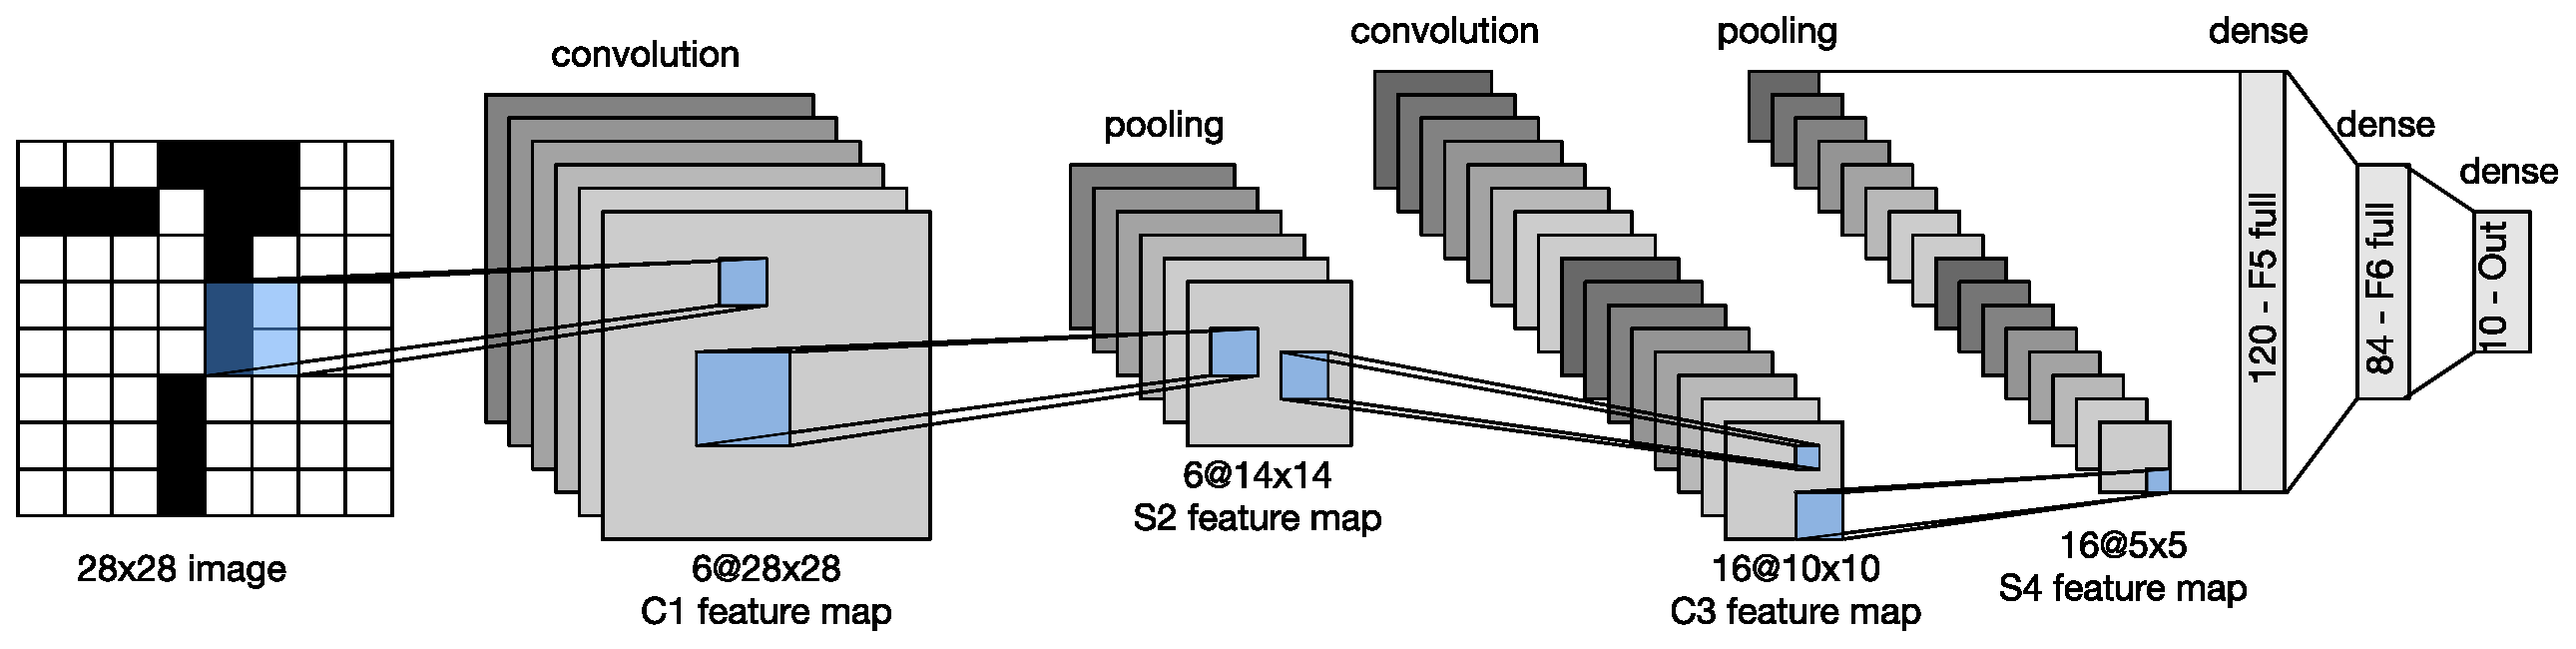
\includegraphics[width=\columnwidth]{images/cnn/lenet.eps}
    \caption{Example of CNN model (LeNet 5)~\cite{CNN}}
    \label{fig:cnn}
\end{figure}

    \chapter{Facial Recognition}\label{ch:face-rec}
Facial recognition is a task of verifying or identifying a person from digital image/video.

As I mentioned in the definition, there are two main subtasks~\cite{FaceRec}:
\begin{enumerate}
    \item \textbf{Verification} deals with verifying whether the person in the image is who he claims he is.
    A typical modern use case of verification is smartphone unlocking with face.
    An example of such system is Face ID developed by Apple Inc.

    \item \textbf{Identification} is a task of matching a person to an identity.
    To formulate it in another way, the goal of identification is to give us an answer to the question of who the person
    in the image is.
\end{enumerate}

\section{Pipeline}\label{sec:pipeline}
Facial recognition pipeline\footnote{\label{foot:pipe}A chain of processing elements, arranged so that the output of
each element is the input of the next.} usually has the following four steps:
\begin{enumerate}
    \item The first one is \textbf{face detection}.
    As the name implies, it deals with the determination of face location within the image.
    Usually the output of the algorithm is face coordinates and facial landmarks.
    The landmarks are a set of coordinates marking important points of the face (eyebrows, nose, mouth, \ldots).
    The knowledge of these points is necessary for the following step.
    An example of face detection system is described in section~\ref{sec:face-detection}.
    \item \textbf{Face alignment} is a task of changing the face position in such a way that it resembles the position
    of faces on which the feature extraction model was trained.
    In most of the instances, this step improves the accuracy.
    \item \textbf{Feature extraction} is a process of computing a feature vector\footnote{A feature vector is a vector
    that contains information describing an object's important characteristics.} from the face.
    Architectures of models used for the feature extraction were described in the previous chapter~\ref{ch:cnn}.
    \item \textbf{Feature matching} uses the feature vector from the previous task to classify a person in the image.
    The algorithm uses a database of pre-computed feature vectors and compares them to the newly extracted one.

    If we are dealing with the \textbf{closed-set problem}~\footnote{\label{foot:closedset}Identifying samples which
    were present in the training dataset.}, the identity associated with the feature vector which has
    the smallest distance from the extracted one is considered to be the identity of the person in the image.

    For the \textbf{open-set problem}~\footnote{\label{foot:openset}Identifying samples which were not present in the
    training dataset.}, the process is similar with the difference being an addition of a threshold.
    This thresholds states the maximum distance from the closest pre-computed feature vector for the newly extracted
    vector to still be classified as that identity.
    In case this condition is not met for any of the identities in the database, we establish the vector as a new
    identity.
\end{enumerate}

It is important to note that the second step is not always present and it is deemed unnecessary by some~\cite{FaceNet}.

\section{Face Recognition Systems}\label{sec:systems}
There are two main approaches of training CNNs for face recognition.

The first one is to train a multi-class classifier which can separate identities directly.
An example of such system is DeepFace~\ref{subsec:deepface}.

The second approach is to learn embedding using the triplet loss~\ref{sec:triplet-loss} function or similar.
FaceNet~\ref{subsec:facenet} is an example of a system being trained using the second approach.

\subsection{DeepFace}\label{subsec:deepface}
DeepFace~\cite{DeepFace} is a system developed by FaceBook Inc. in 2014.

The research is notable for its use of advanced alignment technique which consists of three steps:

\begin{enumerate}
    \item \textbf{2D Alignment}

    In this step, the image is aligned in such a way that the fiducial points/landmarks are in a similar position
    to predetermined reference positions.
    To carry out this process it is first necessary to detect the 6 fiducial points/landmarks.
    These points and the reference positions are then used to find the parameters of an affine transformation.
    Applying the transformation to the original image gives us the desired result.
    \item \textbf{3D Alignment}

    In the second step, the image is warped onto a generic 3D shape model.
    This is achieved by localization of 67 fiducial points in the image and then fitting an affine
    camera\footnote{linear mathematical model to approximate the perspective projection followed by an ideal
    pinhole camera.} \textit{P} using the generalized least squares solution and the reference position $x_{3d}$ of
    points on the 3D shape model.

    \item \textbf{Frontalization}

    This is the final step and it consist of a computation and application of a piece-wise affine transformation T from
    $x_{2d}$ source to $\tilde{x_{3d}}$ target.
    The target $\tilde{x_{3d}}$ is a list of positions of reference fiducial points from the previous step enriched with
    residuals \textit{r}.
    These residuals were added to the reference positions $\tilde{x_{3d}}$ to account for non-rigid deformations which
    are not modeled by the affine camera \textit{P}.
    Without these residuals, all faces would be warped into the same shape losing important discriminative factors.
\end{enumerate}

\begin{figure}[H]
    \centering
    \includegraphics[width=\columnwidth]{images/face-recognition/deepface.png}
    \caption{Outline of DeepFace architecture~\cite{DeepFace}}
    \label{fig:deepface}
\end{figure}

There are 9 layers in the model with over 120 million parameters.
The process of classification is visualized in the picture~\ref{fig:deepface}.
The model was trained on more than 4 million images and as the name of the research paper~\cite{DeepFace} implies,
the results (\textbf{97.35\%} on LFW dataset~\ref{subsec:lfw}) almost matched the results of humans (\textbf{97.53\%}
on LFW dataset).


\subsection{FaceNet}\label{subsec:facenet}
FaceNet~\cite{FaceNet} is a system developed by researchers at Google Inc. in 2015.

An interesting innovation of FaceNet is the format of its output.
The output of the network is a vector representing a position in an euclidean space (so called embeddings) instead of a
number representing an identity.
This approach allows for straight-forward implementation of \textit{verification} and
\textit{identification}~\ref{ch:face-rec}.
The implementation of verification involves thresholding the distance between the reference and the newly obtained
embedding; and identification becomes k-NN classification problem.

\begin{figure}[H]
    \centering
    \includegraphics[width=\columnwidth]{images/face-recognition/facenet.png}
    \caption{Outline of FaceNet architecture~\cite{FaceNet}}
    \label{fig:facenet}
\end{figure}

The loss function used to train the model is called \textit{triplet loss}~\ref{sec:triplet-loss}.
Researches at Google came up with a new online method\footnote{Training samples are selected during training.} which
ensures that the difficulty of triplets is rising as the network trains.

The advantages of the model are its accuracy and the compactness of the face representation.
The accuracy exceeded that of human with \textbf{99.63\%} on LFW dataset~\ref{subsec:lfw} and the euclidean space has
only 128 dimensions.

Another advantage is how well the model handles faces which are not in ideal position.
This removed the need for complex preprocessing and face frontalization.
To use proper terms the system is \textit{pose-invariant}.

\subsection{EyeFace SDK}\label{subsec:eyeface}
EyeFace SDK is a library providing face detection, face recognition, etc. developed by Eyedea Recognition s. r. o..
One of the goals of this thesis is to exceed the performance of this commercial algorithm.
The SDK is closed source; therefore, the implementation details are not known.

\section{Face Detection}\label{sec:face-detection}
As I mentioned in the description of a facial recognition pipeline, the goal of face detection is to find the location
of the face within the image.
This is challenging in unconstrained environments due to various poses, illuminations and occlusions.

To not digress too much from the main topic, I will describe only the system which was employed in the experimental
part of this thesis.
The detection algorithm is called MTCNN~\ref{subsec:mtcnn}.

Before going through the process of face detection, it is necessary to describe a method called Non-maximum Suppression.

\subsection{Non-maximum Suppression}\label{subsec:nms}
Non-maximum Suppression (NMS) is a filtering algorithm of overlapping bounding
boxes\footnote{\label{foot:bbox}A rectangle describing face position.}.
NMS consists of five simple steps:
\begin{enumerate}
    \item \label{itm:nmss1}Create a list of proposal bounding boxes ordered by the confidence score.
    \item Select the bounding box with highest confidence score and add it to the filtered list of boxes.
    \item Compute IoU~\ref{fig:iou} between the selected bounding box and all the remaining ones.
    \item Remove all the boxes whose IoU is higher than some predetermined threshold.
    \item Go to~\ref{itm:nmss1} and repeat the process until there are no remaining bounding boxes within the original list.
\end{enumerate}

Having NMS defined we can proceed with actual face detection.

\subsection{MTCNN}\label{subsec:mtcnn}
MTCNN~\cite{MTCNN} stands for Multi-task Cascaded Convolutional Networks.
This model consists of three stages.

\subsubsection{Stage 1}
The first stage is called \textbf{Proposal Network} (P-Net) and its role is to find the candidate windows and their
bounding box regression vectors.
P-Net is fully convolutional neural network.

Before passing the image to P-Net we resize the image to many different sizes.
By doing so we make the model scale-invariant.

Now we feed the images to the net.

The net produces many bounding boxes with a varying confidence.
We parse the output and delete the boxes with low confidence score.

Now we standardize the coordinates by converting the boxes from the coordinate systems of the resized images to
that of the unscaled one.

At this point we run NMS~\ref{subsec:nms} once for every scaled image.
Then we put all the survivors into one list and run NMS once more.

Before passing the boxes to stage 2 we make the boxes square by elongating the shorter sides.

\subsubsection{Stage 2}
The name of the second stage is \textbf{Refined Network} (R-Net).
The purpose of this stage is to filter out a large number of false positives and to calibrate the boxes.

Initially, we take the boxes from the previous stage and copy the pixel values to separate arrays.
In case the box is out of bounds we fill the "empty space" with zeros.

Now we resize all the arrays to have the size of $24 \times 24$ pixels.
We also normalize the pixel values to $<-1; 1>$.

At this point, we feed the images to R-Net and collect the outputs.

The outputs are similar to that of P-Net.
They also include the coordinates and the confidence levels.
The difference is that the new coordinates are more accurate.

In the last few steps of the stage 2, we remove the boxes with a lower confidence and perform NMS to remove the
redundant ones.

Now we standardize the coordinates and reshape the bounding boxes to a square.

\subsubsection{Stage 3}
In the last stage, we take the boxes from the stage 2 and copy the pixel values to separate arrays.
If there are any boxes which cross the image bounds, we deal with them in the same way as in the previous stage,
i.e., we fill the empty space with zeros.

\begin{wrapfigure}[18]{r}{0pt}
\centering
\includegraphics[width=0.6\columnwidth]{images/face-recognition/mtcnn.png}
\caption{MTCNN face detection pipeline~\cite{MTCNN}.}
\label{fig:mtcnn}
\end{wrapfigure}
Now we resize the images to be of $48 \times 48$ pixels and feed them into a neural network called
\textbf{The Output Network} (O-Net).

O-Net is split into three layers at the top and as a result of this architectural choice produces three outputs:
the coordinates of the bounding box, the coordinates of the facial landmarks and the confidence level of each box.

In the final processing step of the whole MTCNN algorithm, we get rid of the boxes with a low confidence score,
we standardize the coordinates of both the landmarks and the boxes, and  we filter the boxes with NMS.


Figure~\ref{fig:mtcnn} is a visualization of this three-stage process.

\section{Datasets}\label{sec:datasets}
In this section, I will briefly describe datasets used for training and evaluation of facial recognition models.
There are too many different datasets used in practice.
For this reason, I will focus only on those mentioned in this text.

\subsection{LFW}\label{subsec:lfw}
LFW is an acronym for Labeled Faces in the Wild~\cite{LFW}.
The dataset contains 13,000 images and 1680 identities.
Every identity is represented by at least two samples.
The faces were detected by Viola-Jones face detector\footnote{Real-time object detection framework.}.

There are now four publicly used versions of the dataset.
These versions are differentiated by the type of preprocessing (different methods of alignment) applied to the images.

\subsection{YTF}\label{subsec:ytf}
YTF stands for YouTube Faces~\cite{YTF}.
The data set contains 3425 videos and 1,595 unique identities.
The average length of the video clip is 181.3 frames and there are on average 2.15 videos for each subject.

\subsection{MS-Celeb-1M}\label{subsec:ms1m}
MS-Celeb-1M is a dataset constructed by Microsoft Research~\cite{MSCeleb1M}.
There are 10 million face images with nearly 100,000 individuals.
The data were harvested from the Internet.

Due to the method with which the images were collected, there are many mislabellings in the dataset.
For this reason, there are different versions available on the Internet containing refined data (like MS1MV2).

As the name implies, the dataset contains images of celebrities.
In this context, celebrity is assumed to be anyone with frequent online presence.
This became a controversial issue, and as a result, Microsoft pulled the dataset off the Internet.

\subsection{CASIA WebFace}\label{subsec:casia}
CASIA WebFace~\cite{Casia} is a dataset used for scientific research of unconstrained face recognition.
There are approximately 500,000 images and more than 10,000 identities in the database.
The images were crawled~\footnote{Automatically located and downloaded from the Internet.} from the Internet
by Institute of Automation, Chinese Academy of Sciences.

\subsection{Czech News}\label{subsec:czenew}
\begin{wrapfigure}[18]{r}{0pt}
    \centering
    \raisebox{0pt}[\dimexpr\height-0.831\baselineskip\relax]{%
    \begin{forest}
        for tree={
        font=\ttfamily,
        grow'=0,
        child anchor=west,
        parent anchor=south,
        anchor=west,
        calign=first,
        edge path={
        \noexpand\path [draw, \forestoption{edge}]
        (!u.south west) +(7.5pt,0) |- node[fill,inner sep=1.25pt] {} (.child anchor)\forestoption{edge label};
        },
        before typesetting nodes={
        if n=1
        {insert before={[,phantom]}}
        {}
        },
        fit=band,
        before computing xy={l=15pt},
        }
        [annotations
        [name1
        [detections
        [detection1
        [bounding\_box]
        [frame\_number]
        ]
        [detection2
        [bounding\_box]
        [frame\_number]
        ]
        [\ldots]
        ]
        ]
        [name2
        [detections
        [detection1
        [bounding\_box]
        [frame\_number]
        ]
        [\ldots]
        ]
        ]
        [\ldots]
        ]
    \end{forest}
    }
    \caption{Format of annotations}
    \label{fig:annotations}
\end{wrapfigure}
Czech News is a dataset which was created from the recordings of evening news on the czech public television broadcast
(Česká Televize).
The dataset consists of 15 videos and the same amount of annotation files in \textit{json}\footnote{An
open-standard file format that uses human-readable text to transmit data objects consisting of attribute–value pairs
and array data types.} format.

In every annotation file (visualized in figure~\ref{fig:annotations}), there is a dictionary object,
where key is a name, and value is a list of detections.
Every detection contains information about the frame (frame number) and the position of the face (bounding box).
This information is later used to process the dataset (section~\ref{sec:data-preprocessing}).
The reference face position was selected by a human.

In the dataset there are 1238 identities and 732607 detections.

As I mentioned in the section about EyeFace SDK~\ref{subsec:eyeface}, this dataset is used to evaluate my
implementation of the face recognition algorithm (chapter~\ref{ch:implementation}).

    \chapter{ArcFace}\label{ch:arcface}
ArcFace~\cite{ArcFace} is a research which became public in 2018 and achieved state-of-the-art results on LFW dataset.
The objective of the research was to design a loss function which solves the main drawbacks of \textit{sofmax loss}
and the \textit{triplet loss}.

There are two issues with \textit{softmax loss}.
The first one is that the dimension of the output weight matrix grows linearly with the number of identities in the
training set.
The second drawback is that the learned features are not discriminative enough for the open-set face recognition
problem.
That means that the model doesn't perform well on not yet seen faces.

The drawbacks of \textit{triplet loss} are the demands entailed by the construction of the triplets.
The number of those is subject to combinatorial explosion.
This is a serious issue especially for large datasets.


\begin{figure}[H]
    \centering
    \includegraphics[width=\columnwidth]{images/arcface/arcface.png}
    \caption{Training a CNN for face recognition supervised by the ArcFace loss~\cite{ArcFace}}
    \label{fig:arcface}
\end{figure}

%    \setquotestyle{english} % Question marks in place of quotes bug fix
    \printbibliography

\end{document}